\documentclass[11pt,a4paper]{article}

% ─── Packages ────────────────────────────────────────────────────────────────
\usepackage[utf8]{inputenc}
\usepackage[T1]{fontenc}
\usepackage{lmodern}
\usepackage[margin=2.4cm]{geometry}
\usepackage{fancyhdr}
\usepackage{hyperref}
\usepackage{xcolor}
\usepackage[most]{tcolorbox}
\usepackage{booktabs}
\usepackage{longtable}
\usepackage{enumitem}
\usepackage{tikz}
\usetikzlibrary{
  positioning,
  arrows.meta,
  shapes.geometric,
  shapes.multipart,
  fit,
  calc,
  backgrounds,
  decorations.pathreplacing
}
\usepackage{listings}
\usepackage{microtype}

% ─── Colors ──────────────────────────────────────────────────────────────────
\definecolor{ethblue}{RGB}{31,64,122}
\definecolor{swissred}{RGB}{200,40,40}
\definecolor{softgreen}{RGB}{40,140,60}
\definecolor{softpurple}{RGB}{100,50,150}
\definecolor{warmgray}{RGB}{245,242,238}
\definecolor{codebg}{RGB}{248,248,248}
\definecolor{noteyellow}{RGB}{255,248,220}
\definecolor{warnorange}{RGB}{255,240,220}

% ─── tcolorbox styles ───────────────────────────────────────────────────────
\newtcolorbox{conceptbox}[1][]{
  colback=blue!4, colframe=ethblue, fonttitle=\bfseries,
  title=#1, boxrule=0.6pt, arc=2pt, left=6pt, right=6pt,
  top=4pt, bottom=4pt
}

\newtcolorbox{modulebox}[1][]{
  colback=warmgray, colframe=ethblue!70!black, fonttitle=\bfseries,
  title=#1, boxrule=0.5pt, arc=2pt, left=6pt, right=6pt,
  top=4pt, bottom=4pt
}

\newtcolorbox{experimentbox}[1][]{
  colback=green!3, colframe=softgreen!80!black, fonttitle=\bfseries,
  title=#1, boxrule=0.6pt, arc=2pt, left=6pt, right=6pt,
  top=4pt, bottom=4pt
}

\newtcolorbox{notebox}[1][]{
  colback=noteyellow, colframe=orange!70!black, fonttitle=\bfseries,
  title=#1, boxrule=0.5pt, arc=2pt, left=6pt, right=6pt,
  top=4pt, bottom=4pt
}

\newtcolorbox{warnbox}[1][]{
  colback=warnorange, colframe=swissred!80!black, fonttitle=\bfseries,
  title=#1, boxrule=0.6pt, arc=2pt, left=6pt, right=6pt,
  top=4pt, bottom=4pt
}

\newtcolorbox{codebox}[1][]{
  colback=codebg, colframe=black!30, fonttitle=\bfseries\ttfamily,
  title=#1, boxrule=0.4pt, arc=1pt, left=4pt, right=4pt,
  top=3pt, bottom=3pt
}

% ─── Listings ────────────────────────────────────────────────────────────────
\lstset{
  basicstyle=\small\ttfamily,
  backgroundcolor=\color{codebg},
  breaklines=true,
  frame=none,
  columns=fullflexible,
  keepspaces=true,
  showstringspaces=false
}

% ─── Header / Footer ────────────────────────────────────────────────────────
\pagestyle{fancy}
\fancyhf{}
\fancyhead[L]{\small\textsc{LLM Judge Bias/Sensitivity Pipeline}}
\fancyhead[R]{\small\textsc{Architecture Document}}
\fancyfoot[C]{\thepage}
\renewcommand{\headrulewidth}{0.4pt}
\renewcommand{\footrulewidth}{0pt}

% ─── Hyperref ────────────────────────────────────────────────────────────────
\hypersetup{
  colorlinks=true,
  linkcolor=ethblue,
  urlcolor=swissred,
  citecolor=softgreen,
  pdftitle={LLM Judge Bias/Sensitivity Pipeline -- Architecture},
  pdfauthor={ETH Zurich},
}

% ─── Title ───────────────────────────────────────────────────────────────────
\title{%
  \vspace{-1cm}
  \textbf{LLM Judge Bias and Sensitivity}\\[4pt]
  \Large Inference Pipeline Architecture Document\\[6pt]
  \normalsize Swiss AI Stack \,$\cdot$\, Qwen3-30B-A3B-Instruct-2507
}
\author{ETH Z\"urich -- Training Better Preference Models}
\date{March 2026}

% ═════════════════════════════════════════════════════════════════════════════
\begin{document}
\maketitle
\thispagestyle{fancy}
\tableofcontents
\newpage

% ─────────────────────────────────────────────────────────────────────────────
\section{Overall Architecture}\label{sec:architecture}
% ─────────────────────────────────────────────────────────────────────────────

\begin{conceptbox}[Design Philosophy]
The pipeline is a \textbf{pure HTTP client} that sends judge queries to the
\textbf{Swiss AI Stack} (\url{https://serving.swissai.svc.cscs.ch/v1}).
There is no local cluster, no Slurm scheduler, and no local vLLM instance.
All inference is performed remotely via OpenAI-compatible REST requests;
the local code handles only data loading, prompt construction, async
dispatch, response parsing, and metric computation.
\end{conceptbox}

\begin{notebox}[Key Terminology]
\begin{description}[nosep, leftmargin=1.5cm]
  \item[System prompt] A hidden instruction sent to the model \emph{before}
    the user's message. It sets the model's role and behaviour --- for example,
    ``You are an expert rater.'' The user never sees this text; it tells the
    model \emph{how} to act. In this pipeline, the system prompt defines the
    judge persona and output format.
  \item[User prompt] The visible message that the model responds to. It
    contains the actual content to evaluate: the original user question and
    the two candidate responses (A and B). The model reads both the system
    prompt and the user prompt, but only the user prompt carries the data.
\end{description}

\medskip
\noindent Every API call in this pipeline sends exactly one system prompt and one user
prompt. The system prompt varies across experiments (different templates), while
the user prompt varies across dataset pairs (different questions and responses).
\end{notebox}

\subsection{Data-Flow Diagram}

\begin{center}
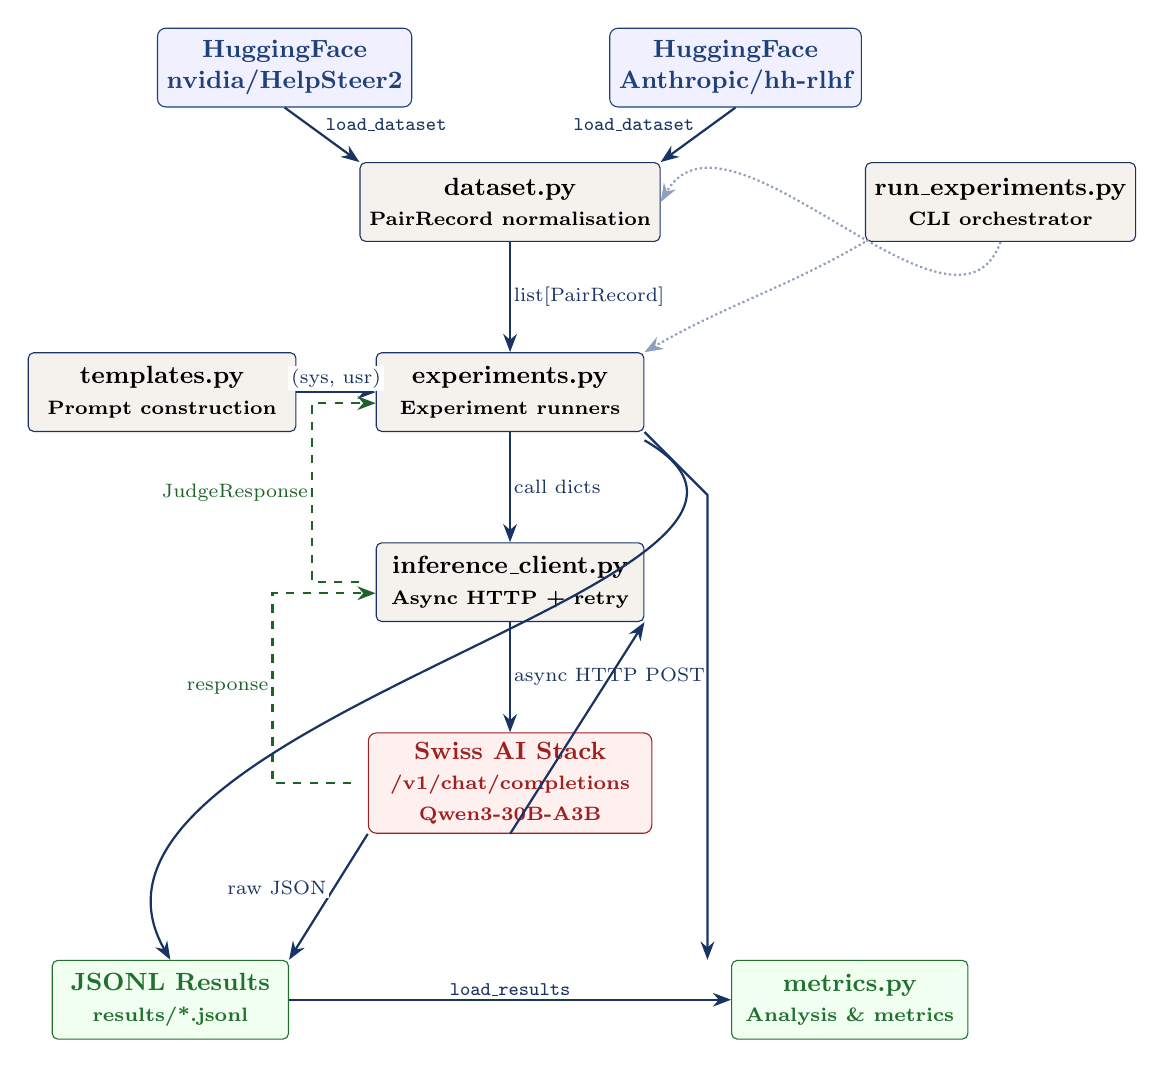
\begin{tikzpicture}[
  >=Stealth,
  node distance=1.0cm and 1.6cm,
  % --- node styles ---
  datasrc/.style={
    draw=ethblue, fill=blue!6, rounded corners=3pt,
    minimum width=3.0cm, minimum height=1.0cm,
    font=\small\bfseries, align=center, text=ethblue
  },
  module/.style={
    draw=ethblue!80!black, fill=warmgray, rounded corners=2pt,
    minimum width=3.4cm, minimum height=1.0cm,
    font=\small\bfseries, align=center
  },
  api/.style={
    draw=swissred!80!black, fill=red!6, rounded corners=3pt,
    minimum width=3.6cm, minimum height=1.1cm,
    font=\small\bfseries, align=center, text=swissred!80!black
  },
  output/.style={
    draw=softgreen!80!black, fill=green!6, rounded corners=2pt,
    minimum width=3.0cm, minimum height=1.0cm,
    font=\small\bfseries, align=center, text=softgreen!80!black
  },
  arr/.style={->, thick, ethblue!80!black},
  arrlbl/.style={font=\scriptsize, midway, fill=white, inner sep=1pt},
]

% Row 1: Data sources
\node[datasrc] (hf1) {HuggingFace\\nvidia/HelpSteer2};
\node[datasrc, right=2.5cm of hf1] (hf2) {HuggingFace\\Anthropic/hh-rlhf};

% Row 2: dataset.py
\node[module, below=1.2cm of $(hf1)!0.5!(hf2)$] (dataset) {dataset.py\\{\scriptsize PairRecord normalisation}};

% Row 3: templates + experiments
\node[module, below left=1.4cm and 0.8cm of dataset] (templates) {templates.py\\{\scriptsize Prompt construction}};
\node[module, below=1.4cm of dataset] (experiments) {experiments.py\\{\scriptsize Experiment runners}};

% Row 4: inference client
\node[module, below=1.4cm of experiments] (client) {inference\_client.py\\{\scriptsize Async HTTP + retry}};

% Row 5: Swiss AI Stack
\node[api, below=1.4cm of client] (swissai) {Swiss AI Stack\\{\scriptsize /v1/chat/completions}\\{\scriptsize Qwen3-30B-A3B}};

% Row 6: outputs
\node[output, below left=1.6cm and 1.0cm of swissai] (jsonl) {JSONL Results\\{\scriptsize results/*.jsonl}};
\node[output, below right=1.6cm and 1.0cm of swissai] (metrics) {metrics.py\\{\scriptsize Analysis \& metrics}};

% Row 7: CLI
\node[module, above right=1.4cm and 2.8cm of experiments] (cli) {run\_experiments.py\\{\scriptsize CLI orchestrator}};

% ─── Arrows ──────────────────────────────────────────────────────────────
\draw[arr] (hf1.south) -- (dataset.north west) node[arrlbl, above right] {\texttt{load\_dataset}};
\draw[arr] (hf2.south) -- (dataset.north east) node[arrlbl, above left] {\texttt{load\_dataset}};
\draw[arr] (dataset.south) -- (experiments.north) node[arrlbl, right] {list[PairRecord]};
\draw[arr] (templates.east) -- (experiments.west) node[arrlbl, above] {(sys, usr)};
\draw[arr] (experiments.south) -- (client.north) node[arrlbl, right] {call dicts};
\draw[arr] (client.south) -- (swissai.north) node[arrlbl, right] {async HTTP POST};
\draw[arr] (swissai.south west) -- (jsonl.north east) node[arrlbl, above left=-1pt] {raw JSON};
\draw[arr] (swissai.south) -- (client.south east) node {} ;

% Return path: SwissAI -> client -> experiments -> JSONL
\draw[arr, dashed, softgreen!70!black]
  ([xshift=-6pt]swissai.west) -- +(-1.0,0) |- ([yshift=-4pt]client.west)
  node[arrlbl, pos=0.25, left] {response};
\draw[arr, dashed, softgreen!70!black]
  ([xshift=-6pt]client.west) -- +(-0.6,0) |- ([yshift=-4pt]experiments.west)
  node[arrlbl, pos=0.25, left] {JudgeResponse};

\draw[arr] (experiments.south east) -- ++(0.8,-0.8) -- (jsonl.north -| {$(experiments.south east)+(0.8,-0.8)$})
  node {} ;
\draw[arr] ([yshift=-3pt]experiments.south east) to[out=-30, in=120] (jsonl.north);

\draw[arr] (jsonl.east) -- (metrics.west) node[arrlbl, above] {\texttt{load\_results}};

% CLI orchestration arrows
\draw[arr, densely dotted, ethblue!50] (cli.south west) to[out=210,in=30] (experiments.north east);
\draw[arr, densely dotted, ethblue!50] (cli.south) to[out=250,in=60] (dataset.east);

\end{tikzpicture}
\end{center}

\begin{notebox}[Data-Flow Summary]
\begin{enumerate}[leftmargin=*, nosep]
  \item \textbf{dataset.py} loads from HuggingFace (HelpSteer2 or hh-rlhf),
        normalises each sample to a \texttt{PairRecord} (prompt\_id, prompt,
        response\_a, response\_b, gold\_label).
  \item \textbf{experiments.py} builds judge call lists from pairs and template
        configurations, dispatches them via \texttt{SwissAIClient.batch\_judge}.
        For example, the position bias experiment creates two calls per pair ---
        one in the original A/B order and one flipped --- producing a list of
        dictionaries like \texttt{\{system\_prompt: ..., user\_prompt: ...,
        prompt\_id: "a3f8", condition: "AB"\}}.
  \item \textbf{inference\_client.py} sends async HTTP POST requests to the
        Swiss AI Stack's OpenAI-compatible \texttt{/v1/chat/completions}
        endpoint.
  \item Responses are parsed using pattern matching (the code searches the
        model's output for verdict lines like ``Verdict: A'' or a standalone
        A/B/C at the end of the text), saved to JSONL, and fed to
        \textbf{metrics.py} for analysis.
\end{enumerate}
\end{notebox}


% ─────────────────────────────────────────────────────────────────────────────
\newpage
\section{Module Responsibilities}\label{sec:modules}
% ─────────────────────────────────────────────────────────────────────────────

% ── inference_client.py ─────────────────────────────────────────────────────
\subsection{inference\_client.py}

\begin{modulebox}[Async HTTP Client for the Swiss AI Stack]
Wraps the remote OpenAI-compatible endpoint with structured request/response
handling, concurrency control, and robust retry logic.
\end{modulebox}

\subsubsection*{Key Components}

\begin{description}[style=nextline, leftmargin=1.5cm]
  \item[\texttt{InferenceConfig}]
    Dataclass holding all configuration:
    \begin{itemize}[nosep]
      \item \texttt{base\_url}: \url{https://serving.swissai.svc.cscs.ch/v1}
      \item \texttt{api\_key}: Bearer token (from \texttt{SWISSAI\_API\_KEY} env var)
      \item \texttt{model}: \texttt{Qwen/Qwen3-30B-A3B-Instruct-2507}
      \item Generation params: \texttt{max\_tokens=2048}, \texttt{temperature=0.0}, \texttt{top\_p=1.0}
      \item Retry config: \texttt{max\_retries=5}, \texttt{retry\_base\_delay=2.0s}, \texttt{retry\_max\_delay=60.0s}
      \item Concurrency: \texttt{concurrent\_requests=8}
    \end{itemize}

  \item[\texttt{JudgeResponse}]
    Dataclass for structured results:
    \texttt{prompt\_id}, \texttt{experiment\_id}, \texttt{condition},
    \texttt{raw\_text}, \texttt{label} (A/B/C/null), \texttt{thinking}
    (extracted CoT or null), \texttt{latency\_s}, \texttt{total\_tokens},
    \texttt{parse\_ok}, \texttt{error}.

  \item[Label Extraction]
    Three-tier pattern-matching cascade (the code searches the model's output
    text for specific formats, trying each rule in order until one matches):
    \begin{enumerate}[nosep]
      \item \textbf{Verdict lines}: looks for explicit markers like
            ``Verdict: B'', ``Answer: A'', ``Output: C''
      \item \textbf{Bare label}: a single A, B, or C standing alone at the
            end of the text
      \item \textbf{Fallback}: scans the entire text and picks the last
            standalone uppercase A, B, or C found
    \end{enumerate}
    If the model produced a \texttt{<think>...</think>} block (internal
    reasoning), that block is stripped before label extraction and stored
    separately in the result.

  \item[\texttt{SwissAIClient}]
    Async context manager creating an \texttt{aiohttp.ClientSession} with
    300\,s timeout. Uses \texttt{asyncio.Semaphore} for concurrency limiting.
    The \texttt{judge()} method sends a single judge call; \texttt{batch\_judge()}
    dispatches a list of calls via \texttt{asyncio.gather}.
\end{description}


% ── templates.py ────────────────────────────────────────────────────────────
\subsection{templates.py}

\begin{modulebox}[Judge Prompt Templates]
Defines all system-prompt variants, criteria, and the shared user-prompt
builder. Each template is registered in the \texttt{TEMPLATES} dictionary.
\end{modulebox}

\subsubsection*{System Prompt Variants}

\begin{center}
\small
\begin{tabular}{lll}
  \toprule
  \textbf{ID} & \textbf{Framing} & \textbf{Used In} \\
  \midrule
  \texttt{expert\_rater}  & Baseline expert rater   & B1, B2, B3, B4 \\
  \texttt{llm\_judge}     & ``LLM used to judge''   & B2 \\
  \texttt{neutral}        & Imperative, no persona  & B2 \\
  \texttt{academic}       & Formal quality evaluator & B2 \\
  \texttt{minimal}        & One-liner               & B2 \\
  \texttt{reason\_then\_judge} & Explain reasoning, then verdict & B3 \\
  \texttt{structured\_reasoning} & Rate on criteria, then verdict & B3 \\
  \texttt{expert\_rater\_alt1} & ``superior response'' & B4 \\
  \texttt{expert\_rater\_alt2} & ``AI-generated answers / preferable'' & B4 \\
  \texttt{expert\_rater\_alt3} & ``serves the user'' & B4 \\
  \bottomrule
\end{tabular}
\end{center}

\subsubsection*{Criteria Variants}

Five criteria defined in the \texttt{CRITERIA} dict: \texttt{helpful},
\texttt{quality}, \texttt{accurate}, \texttt{harmless}, \texttt{concise}.
Each maps to a natural-language fragment (e.g.\ ``more helpful to the user'').

\subsubsection*{\texttt{build\_prompt()}}

Resolves a \texttt{template\_id} + \texttt{criterion} into a
\texttt{(system\_prompt, user\_prompt)} tuple. The user prompt follows a
fixed structure:

\begin{codebox}[\small User Prompt Format]
\begin{lstlisting}
[User Prompt]
{prompt}

[Response A]
{response_a}

[Response B]
{response_b}

Which response is {criterion}?
\end{lstlisting}
\end{codebox}


% ── dataset.py ──────────────────────────────────────────────────────────────
\subsection{dataset.py}

\begin{modulebox}[Dataset Loading and Normalisation]
Loads HuggingFace preference datasets and normalises them into a unified
\texttt{PairRecord} format suitable for pairwise judge evaluation.
\end{modulebox}

\subsubsection*{\texttt{PairRecord} Dataclass}

\begin{description}[style=nextline, leftmargin=1.5cm, nosep]
  \item[\texttt{prompt\_id}] Unique identifier (MD5 hash or index-based)
  \item[\texttt{prompt}] The original user query
  \item[\texttt{response\_a}] First response (chosen / higher-rated in original data)
  \item[\texttt{response\_b}] Second response (rejected / lower-rated)
  \item[\texttt{gold\_label}] ``A'', ``B'', or ``C'' derived from human preference
\end{description}

The \texttt{flipped()} method returns a new record with A/B swapped and the
gold label adjusted (\texttt{A}$\leftrightarrow$\texttt{B}, \texttt{C} unchanged).

\subsubsection*{Dataset Loaders}

\begin{description}[style=nextline, leftmargin=1.5cm]
  \item[HelpSteer2 (\texttt{nvidia/HelpSteer2})]
    A scored (not pairwise) dataset. Pairs are constructed by grouping
    responses by prompt and taking the highest-scored vs.\ lowest-scored
    response. Score = mean(helpfulness + correctness + coherence) / 3.

  \item[HH-RLHF (\texttt{Anthropic/hh-rlhf})]
    A pairwise dataset with chosen/rejected columns. The loader extracts
    the last assistant turn from each multi-turn conversation. Gold label
    is always ``A'' (chosen is preferred).
\end{description}


% ── experiments.py ──────────────────────────────────────────────────────────
\subsection{experiments.py}

\begin{modulebox}[Experiment Runners (B1--B4)]
Four async functions, each building call dicts, dispatching via
\texttt{batch\_judge}, and saving JSONL results. Contains condition
definitions for each experiment.
\end{modulebox}

\begin{center}
\small
\begin{tabular}{llp{6.5cm}}
  \toprule
  \textbf{Function} & \textbf{ID} & \textbf{Conditions} \\
  \midrule
  \texttt{run\_position\_bias}       & B1 & ``AB'' (original), ``BA'' (flipped) \\
  \texttt{run\_template\_sensitivity}& B2 & 5 templates: expert\_rater, llm\_judge, neutral, academic, minimal \\
  \texttt{run\_reasoning\_depth}     & B3 & 3 conditions: no\_reasoning, reason\_then\_judge, structured\_reasoning \\
  \texttt{run\_input\_sensitivity}   & B4 & 4 templates $\times$ 5 criteria = 20 conditions \\
  \bottomrule
\end{tabular}
\end{center}

\subsubsection*{How Call Lists Are Built --- Worked Example}

Each experiment loops over pairs (and conditions) to build a flat list of
dictionaries. Each dictionary contains everything needed for one API call.
Here is a simplified example for position bias (B1) with 2 pairs:

\begin{codebox}[\small B1 Call List Construction (Pseudocode)]
\begin{lstlisting}
pairs = [pair_1, pair_2]   # loaded from dataset

calls = []
for pair in pairs:
    # Original order: Response A first, Response B second
    sys_prompt, usr_prompt = build_prompt("expert_rater",
        pair.prompt, pair.response_a, pair.response_b)
    calls.append({
        "system_prompt": sys_prompt,
        "user_prompt":   usr_prompt,
        "prompt_id":     pair.prompt_id,
        "condition":     "AB"
    })

    # Flipped order: Response B first, Response A second
    flipped = pair.flipped()
    sys_prompt, usr_prompt = build_prompt("expert_rater",
        flipped.prompt, flipped.response_a, flipped.response_b)
    calls.append({
        "system_prompt": sys_prompt,
        "user_prompt":   usr_prompt,
        "prompt_id":     pair.prompt_id,
        "condition":     "BA"
    })

# Result: 4 calls (2 pairs x 2 orders)
# All dispatched at once via client.batch_judge(calls)
\end{lstlisting}
\end{codebox}

For B2, the outer loop iterates over 5 templates instead of 2 orders.
For B3, it iterates over 3 reasoning conditions.
For B4, it iterates over 4 template variants $\times$ 5 criteria = 20 combinations.


% ── metrics.py ──────────────────────────────────────────────────────────────
\subsection{metrics.py}

\begin{modulebox}[Metric Computation and Reporting]
Loads JSONL results and computes experiment-specific metrics. Provides
\texttt{print\_summary()} for console output.
\end{modulebox}

\begin{description}[style=nextline, leftmargin=1.5cm]
  \item[\texttt{compute\_position\_bias}] Position consistency, bias rates,
    positional preference breakdown.
  \item[\texttt{compute\_pairwise\_agreement}] Overall pairwise agreement,
    per-pair agreement rate, label distribution per condition, most volatile
    pairs. Used for both B2 and B4.
  \item[\texttt{compute\_thinking\_accuracy}] Accuracy vs.\ gold labels per
    condition, agreement vs.\ no\_reasoning baseline, average latency per
    condition. Used for B3.
\end{description}


% ── run_experiments.py ──────────────────────────────────────────────────────
\subsection{run\_experiments.py}

\begin{modulebox}[CLI Orchestrator]
Top-level entry point with \texttt{argparse}. Loads dataset, configures
the inference client, runs selected experiments, computes metrics, and
prints summaries.
\end{modulebox}

\begin{codebox}[\small Example Invocations]
\begin{lstlisting}
# Run all experiments (200 pairs, default settings)
python3 run_experiments.py

# Quick smoke test: position bias only, 20 pairs
python3 run_experiments.py --experiments position_bias --n-pairs 20

# Run only reasoning depth experiment
python3 run_experiments.py --experiments reasoning_depth

# Full configuration
python3 run_experiments.py --dataset nvidia/HelpSteer2 \
    --split validation --n-pairs 200 --criterion helpful
\end{lstlisting}
\end{codebox}

CLI flags include: \texttt{--experiments}, \texttt{--n-pairs},
\texttt{--dataset}, \texttt{--split}, \texttt{--criterion},
\texttt{--template}, \texttt{--output-dir},
\texttt{--model}, \texttt{--base-url}, \texttt{--concurrency},
\texttt{--seed}.


% ─────────────────────────────────────────────────────────────────────────────
\newpage
\section{The Four Experiments}\label{sec:experiments}
% ─────────────────────────────────────────────────────────────────────────────

% ── B1 ──────────────────────────────────────────────────────────────────────
\subsection{B1: Position Bias}\label{sec:b1}

\begin{experimentbox}[B1 -- Position Bias Detection]
\textbf{Research question:} Does the LLM judge prefer whichever response
appears in a particular position (first or second), regardless of content?

\medskip
\textbf{Method:} For each pair, judge both orders:
\begin{itemize}[nosep]
  \item \textbf{AB} (original): Response A first, Response B second
  \item \textbf{BA} (flipped): Response B first, Response A second
\end{itemize}
A \emph{consistent} judge should prefer the same underlying response in both
orderings. If the AB verdict is ``A'', the BA verdict should be ``B''
(the same response, now in position B).

\medskip
\textbf{Metrics:}
\begin{description}[nosep, leftmargin=1.2cm]
  \item[\texttt{position\_consistency}] Percentage of pairs where the flipped
    label matches the expected inversion.
  \item[\texttt{position\_bias\_rate}] $1 - \text{consistency}$; the fraction
    where the model's verdict changed with position.
  \item[\texttt{bias\_toward\_first\_position}] Both AB and BA say ``A''
    (always picks first).
  \item[\texttt{bias\_toward\_second\_position}] Both AB and BA say ``B''
    (always picks second).
\end{description}
\end{experimentbox}


% ── B2 ──────────────────────────────────────────────────────────────────────
\subsection{B2: Template Sensitivity}\label{sec:b2}

\begin{experimentbox}[B2 -- Template Sensitivity Analysis]
\textbf{Research question:} How sensitive is the judge's verdict to the
framing of the system prompt, given identical data and response ordering?

\medskip
\textbf{Method:} Judge each pair with 5 different system prompt templates:

\begin{center}
\small
\begin{tabular}{ll}
  \toprule
  \textbf{Template} & \textbf{Character} \\
  \midrule
  \texttt{expert\_rater} & ``You are an expert rater\ldots'' \\
  \texttt{llm\_judge}    & ``You are an LLM used to judge\ldots'' \\
  \texttt{neutral}       & ``Compare the following two responses\ldots'' \\
  \texttt{academic}      & ``You are a quality evaluator\ldots'' \\
  \texttt{minimal}       & ``Pick the better response: A, B, or C (tie).'' \\
  \bottomrule
\end{tabular}
\end{center}

Same data, same order, same criterion --- only the system prompt changes.

\medskip
\textbf{Metrics:}
\begin{description}[nosep, leftmargin=1.2cm]
  \item[\texttt{overall\_pairwise\_agreement}] Average pairwise agreement
    across all template pairs for each prompt.
  \item[\texttt{label\_distribution\_per\_condition}] A/B/C breakdown for
    each template.
  \item[\texttt{most\_volatile\_pairs}] The 10 pairs with lowest agreement
    across templates.
\end{description}
\end{experimentbox}


% ── B3 ──────────────────────────────────────────────────────────────────────
\subsection{B3: Prompt-Elicited Reasoning}\label{sec:b3}

\begin{experimentbox}[B3 -- Reasoning Depth]
\textbf{Research question:} Does explicitly asking the model to reason before
giving its verdict improve accuracy against human gold labels?

\medskip
All reasoning in this experiment is \textbf{prompt-elicited}: the prompt
itself tells the model how much (or how little) to reason. There is no
native API thinking-budget feature involved --- the only thing that changes
between conditions is the system prompt template.

\medskip
\textbf{Conditions:}

\begin{center}
\small
\begin{tabular}{lp{8cm}}
  \toprule
  \textbf{Condition} & \textbf{What the prompt tells the model} \\
  \midrule
  \texttt{no\_reasoning} &
    Just output a single letter: A, B, or C. No explanation requested.
    Uses the baseline \texttt{expert\_rater} template. \\[4pt]
  \texttt{reason\_then\_judge} &
    ``Explain your reasoning about the strengths and weaknesses of each
    response, then provide your final verdict.'' The model argues its
    decision before answering. \\[4pt]
  \texttt{structured\_reasoning} &
    ``Rate each response on helpfulness, accuracy, and coherence, then
    provide your final verdict.'' The model evaluates on specific criteria
    before deciding. \\
  \bottomrule
\end{tabular}
\end{center}

\medskip
\textbf{Metrics:}
\begin{description}[nosep, leftmargin=1.2cm]
  \item[\texttt{accuracy\_vs\_gold}] Agreement with human preference labels
    per condition.
  \item[\texttt{delta\_accuracy}] Improvement of each reasoning condition
    over \texttt{no\_reasoning}.
  \item[\texttt{agreement\_vs\_no\_reasoning}] Fraction of verdicts matching
    the no-reasoning baseline.
  \item[\texttt{avg\_latency\_s}] Average response time per condition
    (reasoning conditions produce longer outputs and take more time).
\end{description}
\end{experimentbox}

\begin{notebox}[B3 Design Note]
This experiment tests \textbf{prompt-elicited Chain of Thought} --- the model
is explicitly told in the prompt to argue its decision before answering.
This is fundamentally different from a native API thinking-budget feature
(like Anthropic's extended thinking or Qwen3's \texttt{enable\_thinking}
parameter). Here, the reasoning appears directly in the model's visible
output because the \emph{prompt} requested it, not because a special API
mode was activated.
\end{notebox}


% ── B4 ──────────────────────────────────────────────────────────────────────
\subsection{B4: Input Sensitivity}\label{sec:b4}

\begin{experimentbox}[B4 -- Input / Wording Sensitivity]
\textbf{Research question:} How sensitive is the judge to minor paraphrasing
of the system prompt and changes in evaluation criterion?

\medskip
\textbf{Method:} Cross 4 minor wording variants of the expert\_rater
template with 5 evaluation criteria:

\begin{center}
\small
\begin{tabular}{lp{7cm}}
  \toprule
  \textbf{Template Variant} & \textbf{Key Wording Difference} \\
  \midrule
  \texttt{expert\_rater}      & Baseline: ``determine which response is better'' \\
  \texttt{expert\_rater\_alt1} & ``identify the superior response'' \\
  \texttt{expert\_rater\_alt2} & ``AI-generated answers'' + ``which answer is preferable'' \\
  \texttt{expert\_rater\_alt3} & ``Evaluate both\ldots select the one that better serves the user'' \\
  \bottomrule
\end{tabular}
\end{center}

\begin{center}
\small
\begin{tabular}{ll}
  \toprule
  \textbf{Criterion} & \textbf{Phrase} \\
  \midrule
  \texttt{helpful}  & ``more helpful to the user'' \\
  \texttt{quality}  & ``of higher overall quality'' \\
  \texttt{accurate} & ``more accurate and factually correct'' \\
  \texttt{harmless} & ``safer and more appropriate'' \\
  \texttt{concise}  & ``more concise while still fully answering the question'' \\
  \bottomrule
\end{tabular}
\end{center}

Total: $4 \times 5 = 20$ conditions per pair.

\medskip
\textbf{Metrics:}
\begin{description}[nosep, leftmargin=1.2cm]
  \item[\texttt{pairwise\_agreement}] Agreement rate across all 20 conditions.
  \item[\texttt{criterion\_drift}] How much the label changes when only the
    criterion changes (template held fixed).
\end{description}
\end{experimentbox}


% ─────────────────────────────────────────────────────────────────────────────
\newpage
\section{Async Concurrency and Retry/Backoff Logic}\label{sec:concurrency}
% ─────────────────────────────────────────────────────────────────────────────

\begin{conceptbox}[Concurrency Model]
The pipeline uses Python's \texttt{asyncio} event loop with
\texttt{aiohttp} for non-blocking HTTP. All experiment calls are dispatched
simultaneously via \texttt{asyncio.gather}, bounded by a semaphore.
\end{conceptbox}

\subsection{Concurrency Control}

\begin{center}
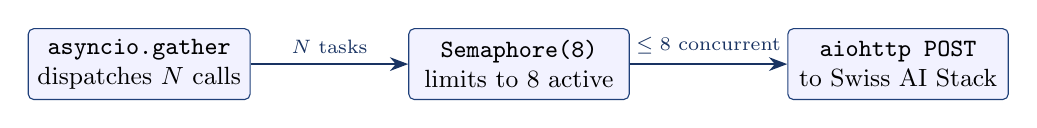
\begin{tikzpicture}[
  >=Stealth,
  box/.style={draw=ethblue, fill=blue!5, rounded corners=2pt,
              minimum width=2.8cm, minimum height=0.9cm,
              font=\small, align=center},
  arr/.style={->, thick, ethblue!80!black},
]

\node[box] (gather) {\texttt{asyncio.gather}\\dispatches $N$ calls};
\node[box, right=2.0cm of gather] (sem) {\texttt{Semaphore(8)}\\limits to 8 active};
\node[box, right=2.0cm of sem] (http) {\texttt{aiohttp POST}\\to Swiss AI Stack};

\draw[arr] (gather) -- (sem) node[midway, above, font=\scriptsize] {$N$ tasks};
\draw[arr] (sem) -- (http) node[midway, above, font=\scriptsize] {$\leq 8$ concurrent};

\end{tikzpicture}
\end{center}

\begin{itemize}[nosep]
  \item \texttt{SwissAIClient} creates an \texttt{aiohttp.ClientSession} as
    an async context manager with a 300\,s total timeout per request.
  \item An \texttt{asyncio.Semaphore(concurrent\_requests)} (default 8)
    ensures no more than 8 HTTP requests are in flight simultaneously.
  \item \texttt{batch\_judge(calls)} wraps all calls in \texttt{asyncio.gather}
    for maximum parallelism within the semaphore bound.
\end{itemize}

\subsection{Exponential Backoff Retry}

\begin{center}
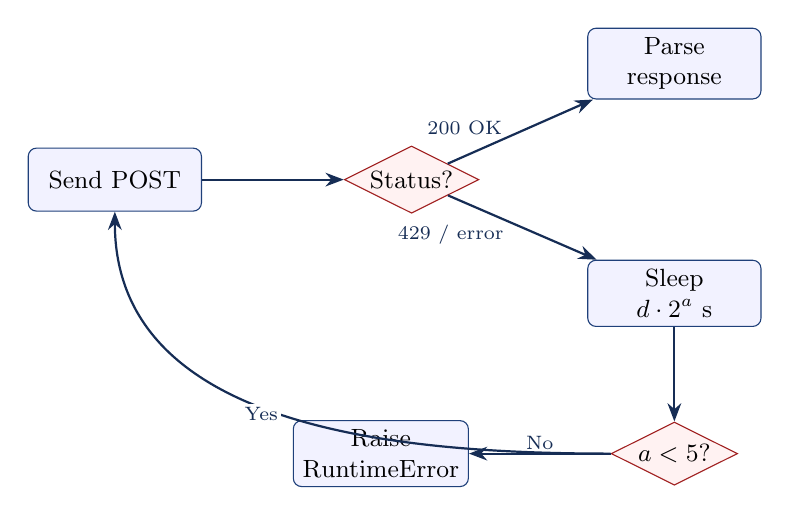
\begin{tikzpicture}[
  >=Stealth,
  state/.style={draw=ethblue, fill=blue!5, rounded corners=3pt,
                minimum width=2.2cm, minimum height=0.8cm,
                font=\small, align=center},
  decision/.style={draw=swissred!80!black, fill=red!5,
                   diamond, aspect=2, inner sep=1pt,
                   font=\small, align=center},
  arr/.style={->, thick, ethblue!70!black},
  lbl/.style={font=\scriptsize, fill=white, inner sep=1pt},
]

\node[state] (req) {Send POST};
\node[decision, right=1.8cm of req] (check) {Status?};
\node[state, above right=0.8cm and 1.8cm of check] (ok) {Parse\\response};
\node[state, below right=0.8cm and 1.8cm of check] (wait) {Sleep\\$d \cdot 2^a$ s};
\node[decision, below=1.2cm of wait] (retry) {$a < 5$?};
\node[state, left=1.8cm of retry] (fail) {Raise\\RuntimeError};

\draw[arr] (req) -- (check);
\draw[arr] (check) -- (ok) node[lbl, pos=0.4, above left] {200 OK};
\draw[arr] (check) -- (wait) node[lbl, pos=0.4, below left] {429 / error};
\draw[arr] (wait) -- (retry);
\draw[arr] (retry.west) -- (fail) node[lbl, midway, above] {No};
\draw[arr] (retry.west) to[out=180, in=270] node[lbl, pos=0.5, left] {Yes} (req.south);

\end{tikzpicture}
\end{center}

\begin{itemize}[nosep]
  \item On HTTP 429 (rate limit) or \texttt{aiohttp.ClientError}, the client
    waits $\min(\texttt{base\_delay} \times 2^{\texttt{attempt}},\;
    \texttt{retry\_max\_delay})$ seconds.
  \item Default: \texttt{base\_delay} = 2.0\,s, \texttt{max\_delay} = 60.0\,s,
    so delays are 2, 4, 8, 16, 32\,s (capped at 60\,s).
  \item After 5 failed attempts, a \texttt{RuntimeError} is raised.
  \item Successful responses (HTTP 200) are parsed immediately; the label
    extractor runs on the response text.
\end{itemize}


% ─────────────────────────────────────────────────────────────────────────────
\newpage
\section{Output JSONL Format}\label{sec:output}
% ─────────────────────────────────────────────────────────────────────────────

\begin{conceptbox}[Result Serialisation]
Each experiment writes one JSONL file to the \texttt{results/} directory.
Each line is a single JSON object representing one judge call.
\end{conceptbox}

\begin{codebox}[\small JSONL Record Schema]
\begin{lstlisting}
{
  "prompt_id":     "a3f8b2c901",
  "experiment_id": "position_bias",
  "condition":     "AB",
  "raw_text":      "Response A is more helpful because...\nVerdict: A",
  "label":         "A",
  "thinking":      null,
  "latency_s":     2.341,
  "total_tokens":  487,
  "parse_ok":      true,
  "error":         null
}
\end{lstlisting}
\end{codebox}

\begin{center}
\small
\begin{longtable}{llp{7cm}}
  \toprule
  \textbf{Field} & \textbf{Type} & \textbf{Description} \\
  \midrule
  \endhead
  \texttt{prompt\_id} & \texttt{str} &
    Unique identifier for the dataset pair (MD5 hash or index-based). \\
  \texttt{experiment\_id} & \texttt{str} &
    Experiment name: \texttt{position\_bias}, \texttt{template\_sensitivity},
    \texttt{reasoning\_depth}, or \texttt{input\_sensitivity}. \\
  \texttt{condition} & \texttt{str} &
    Experimental condition (e.g.\ ``AB'', ``BA'', template name,
    ``reason\_then\_judge'', ``expert\_rater\_alt2\_accurate''). \\
  \texttt{raw\_text} & \texttt{str} &
    Full model output text, unmodified. \\
  \texttt{label} & \texttt{str|null} &
    Extracted verdict: ``A'', ``B'', ``C'', or \texttt{null} if parsing failed. \\
  \texttt{thinking} & \texttt{str|null} &
    Content of \texttt{<think>...</think>} block if present; \texttt{null}
    otherwise. \\
  \texttt{latency\_s} & \texttt{float} &
    Wall-clock time for this request in seconds. \\
  \texttt{total\_tokens} & \texttt{int} &
    Total tokens (prompt + completion) as reported by the API. \\
  \texttt{parse\_ok} & \texttt{bool} &
    Whether label extraction succeeded. \\
  \texttt{error} & \texttt{str|null} &
    Error message if the request failed; \texttt{null} on success. \\
  \bottomrule
\end{longtable}
\end{center}

Results are loaded by \texttt{metrics.py}'s \texttt{load\_results(path)}
function, which reads each line as a JSON object and returns a
\texttt{list[dict]} for downstream analysis.

\subsection*{File Layout}

\begin{codebox}[\small Results Directory Structure]
\begin{lstlisting}
results/
  position_bias/
    expert_rater_helpful.jsonl
  template_sensitivity/
    criterion_helpful.jsonl
  reasoning_depth/
    criterion_helpful.jsonl
  input_sensitivity/
    all.jsonl
\end{lstlisting}
\end{codebox}


% ─────────────────────────────────────────────────────────────────────────────
\newpage
\section{Infrastructure Summary}\label{sec:infra}
% ─────────────────────────────────────────────────────────────────────────────

\begin{warnbox}[No Local Compute]
This pipeline performs \textbf{zero local GPU inference}. All model calls are
HTTP requests to the Swiss AI Stack. The local machine only needs Python 3.10+
with \texttt{aiohttp}, \texttt{datasets}, and \texttt{numpy}.
\end{warnbox}

\begin{center}
\small
\begin{tabular}{ll}
  \toprule
  \textbf{Component} & \textbf{Detail} \\
  \midrule
  Inference backend & Swiss AI Stack (CSCS) \\
  Endpoint URL & \url{https://serving.swissai.svc.cscs.ch/v1} \\
  API compatibility & OpenAI \texttt{/v1/chat/completions} \\
  Model & \texttt{Qwen/Qwen3-30B-A3B-Instruct-2507} \\
  Authentication & Bearer token via \texttt{SWISSAI\_API\_KEY} \\
  Protocol & HTTPS + JSON \\
  Client library & \texttt{aiohttp} (async) \\
  Concurrency & Semaphore-bounded (default 8) \\
  Retry strategy & Exponential backoff, max 5 retries \\
  Local dependencies & Python 3.10+, aiohttp, datasets, numpy \\
  Scheduler / cluster & \textbf{None} (no Slurm, no local vLLM) \\
  \bottomrule
\end{tabular}
\end{center}

% ─────────────────────────────────────────────────────────────────────────────

\vfill
\begin{center}
\small\textit{End of Architecture Document}
\end{center}

\end{document}
